\documentclass[a4paper]{article}
\usepackage[dutch]{babel}
\usepackage{amsmath}
\usepackage{graphicx}
\usepackage{epstopdf}
\usepackage{caption}
\usepackage{subcaption}
\usepackage{courier}

\title{Technisch Wetenschappelijke Software: Project deel 1}
\author{Dries De Samblanx}
\date{dindag 20 november 2015}

\newcommand{\opgave}[1]{\section*{Opgave #1}}
\newcommand{\dx}{\Delta x}
\newcommand{\dy}{\Delta y}
\newcommand{\dz}{\Delta z}
\newcommand{\dt}{\Delta t}

\begin{document}
\maketitle

\begin{abstract}

Dit is het abstract

\end{abstract}

\section*{Methodologie}

\subsection*{ontwerp en datastructuren}

Bij een project van wetenschappelijke software is het belangrijk om niet direct te beginnen met implementeren maar om eerst na te denken over het ontwerp van de implementatie en over de gebruikte datastructuren.\\ 
Een matrix heb ik voorgesteld met behulp van een voorgedefini\"eerd type. Op deze manier is het eenvoudig om met een boolean bij te houden of een matrix volledig of met een rank-k benadering wordt bijgehouden. Daarnaast bevat het type ook twee pointers naar een twee-dimensionale array. Hiermee kan bij het inlezen van de matrix beslist worden of er \'e\'en of twee pointers gealloceerd worden en hoe groot de arrays zijn. Het gebruik van pointers boven allocatable arrays heeft ook voordelen op vlak van geheugengebruik. Bij het berekenen van een product tussen een rank-k matrix en een volledige matrix wordt het resultaat bijvoorbeeld gegeven met behulp van een rank-k matrix. \'e\'en van de twee factoren van deze uitkomst is identiek aan \'e\'en van de twee factoren van de oorspronkelijke rank-k matrix. Door het gebruik van pointers kunnen deze allebei beschreven worden door hetzelfde stuk geheugen, wat niet mogelijk was geweest met een allocatable array. \\
De structuur van de implementatie van het project lag in grote lijnen voor de hand. Het was nodig om een interface te schrijven om alle commando's door te verwijzen naar hun respectievelijke functie. Eerst had ik alle commando's vertaald in kleine programma's die zelf matrices inlazen en wegschreven. Hier ben ik achteraf op teruggekomen door het globale programma verantwoordelijk te maken voor het inlezen en wegschrijven van matrices. Dit vertaalde zich dan in \'e\'en programma dat gebruikmaakte van subroutines die bewerkingen deden op de matrices die zij megekregen hadden. Deze implementatie had niet alleen het voordeel van overzichtelijker te zijn en een indruk te geven van een beter samenhangend geheel, maar bleek ook veel handiger voor het uitvoeren van de tests waar gewerkt moest worden met vooraf ingelezen matrices. 

\subsection*{inlezen en wegschrijven matrices}

De functies die fortran voorziet voor het inlezen en wegschrijven van matrices zijn gemakkelijk en robuust. Omdat deze lijn per lijn inlezen en wegschrijven en omdat fortran column-major orde is, heb ik de keuze gemaakt al de matrices in hun getransponeerde vorm op te slaan. Op deze manier gebeurt het inlezen en het wegschrijven voor grote matrices sneler aangezien de elementen van de matrices op deze manier in dezelfde volgorde worden ingelezen als weggeschreven. Dit resulteert in een grote vermindering van het aantal geheugentoegangen wat een belangrijke vertragende factor is. Alle bewerkingen die op gewone matrices gedaan worden kunnen herleid worden tot bewerkingen op hun transposes. De moeilijkheid die dit met zich meebrengt is het denkwerk. Methodes voor bijvoorbeeld het product van twee rank-k matrices zijn relatief eenvoudig om over te redeneren, maar wanneer men enkel beschikt over de transposes, en ook de transposes van de uitkomstmatrix moet bekomen, moet men heel geconcentreerd blijven om geen fouten te maken. Deze beslissing heeft dan ook heel wat extra denkwerk gekost en een hele tijd extra debug werk. \\
Voor randgevallen zoals de implementatie bij rank-0 matrices moest de compleetheid van de code afgewogen worden tegen de compactheid en de effici\"entie. Om bewerkingen met rank-0 matrices correct af te handelen zijn er echter een hele hoop if-testen nodig op verschillende plaatsen. Aangezien dit ten koste is van zowel de effici\"entie als de leesbaarheid van de code heb ik beslist dit niet te doen. Om toch ongewenste fouten te voorkomen heb ik bij de implementatie van lowrank er voor gezorgd dat er nooit een rank-0 matrix teruggegeven wordt.

\subsection*{matrixbewerkingen}
Alle matrices worden volledig voorgesteld in dubbele precisie. Voor wetenschappelijke software is het belangrijk bewerkingen niet uit te voeren met enkele precisie, maar zeker met dubbele. Uit de oefenzittingen is gebleken dat extended precisie bij de compiler Nagfor bijvoorbeeld verschilt van de extended precisie bij andere compilers. Daarom is heel de implementatie gebeurd met dubbele precisie. Deze beslissing is duidelijk gemaakt door het gebruik van de benaming \verb!double precision! van alle types matrices en re\"ele getallen. Dit maakt het moeilijker om een eventuele overstap te maken naar bijvoorbeeld enkele precisie getallen, maar omdat de code zo leesbaarder is en alle gebruikte subroutines van lapack gemaakt zijn voor dubbele precisie is toch deze formulering gebruikt. \\
Een andere belangrijke beslissing was nodig bij het berekenen van een rank-k benadering van een matrix die ingelezen wordt in rank vorm. De gebruikte implementatie gebruikt geen precondities in verband met de matrices van de rank-k benadering maar is wel niet heel effici\"ent wanneer het op geheugen of snelheid aankomt. De gebruikte methode maakt eerst de volledige matrix met de functie \verb!full! en berekent vervolgens hiervan de rank-k benadering. Wanneer op deze manier een rank-2 benadering wordt gemaakt van een rank-5 (1000x1000) matrix moet wel eerst de volledige 1000x1000 matrix berekend worden. Een andere implementatie zou bijvoorbeeld kunnen veronderstellen dat de gegeven rank matrix de vorm heeft zoals hij uit de methode lowrank zelf zou komen. Dan zou het al voldoende zijn om na te kijken welke kolommen van de matrix A bij de laagste singuliere waarden horen en deze dan samen met hun overeenkomstige kolommen in de B matrix laten vallen. Dit maakt de methode minder robuust maar het zou nog altijd een correcte implementatie zijn voor matrixen gevormd door de applicatie zelf. Daarnaast zou dit veel sneller en veel geheugen effici\"enter zijn. Met deze laatste methode heeft de gebruiker nog altijd de mogelijkheid via het programma eerst zelf de volledige matrix te berekenen en hierna een nieuwe rank-k benadering te maken.

\subsection*{integraal vergelijking}

Voor het opstellen van de matrix A bij het commando makeGFull is de formule op een aangepaste versie ge\"implementeerd.
\begin{equation}
\label{matA}
\begin{aligned}
	&A_{i,j} = -ln( \\ &\sqrt[]{(cos(2\pi (j+0.5)/N)-cos(2\pi i/N))^2
	 +(sin(2\pi (j+0.5)/N)-sin(2\pi i/N))^2})
\end{aligned}
\end{equation}
We kunnen hierbij de twee kwadraten uitwerken en de log van een vierkantswortel schrijven als de halve log.
\begin{equation}
\label{matAvoluit}
\begin{aligned}
	A_{i,j} = & -0.5ln((cos(2\pi (j+0.5)/N)^2-2cos(2\pi i/N)cos(2\pi (j+0.5)/N) \\ & + cos(2\pi i/n)^2
	 +(sin(2\pi (j+0.5)/N)^2 \\ & -2sin(2\pi i/N)sin(2\pi (j+0.5)/N)+sin(2\pi i/N)^2)
\end{aligned}
\end{equation}
Nu kunnen we ook nog tweemaal gebruik maken van de grondformule van de goniometrie en van de dubbele cosinus regel.
\begin{equation}
\label{matAkort}
\begin{aligned}
	A_{i,j} = -0.5ln(2 - 2cos((1+2j-2i)\pi/N))
\end{aligned}
\end{equation}
Hieraan kunnen we ook zien dat alle kolommen van deze matrix kopie\"en zijn val elkaar, enkel \"e\"en plaats naar onder geshift per kolom. Op dezelfde manier kunnen we de sommatie voor $u_N(x)$ herschrijven.
\begin{equation}
\label{un}
\begin{aligned}
	u_N(x) = -\sum_{j=0}^{N-1} 0.5c_jln(1+x_1^2+x_2^2 &-2x_1cos(2\pi (j+0.5)/N)\\&-2x_2sin(2\pi (j+0.5)/N))
\end{aligned}
\end{equation}
Op deze manier proberen we de effici\"entie en nauwkeurigheid van het opstellen van de matrix A en de vector u te verbeteren.

\subsection*{tests}
Bij het uitvoeren van de tests voor het bepalen van de twee reeksen ontstaan er problemen bij het dealloceren van matrices. Door het gebruik van valgrind is het duidelijk dat er bij enkele bewerkingen geen geheugenlekken aanwezig zijn. Bij de tests worden echter dezelfde matrices gebruikt voor meerdere achtereenvolgende bewerkingen op te doen. Wanneer ik hier probeer om de matrices te deallocaren komen er fouten naar boven. Als ik prints doe tussen elke regel in de functie \verb! M_dealloc! in het bestand \(matrixConverter.f90\) geeft hij weer dat de matrix gealloceerd is, maar geeft hij een error omdat hij een matrix geen twee keer kan dealloceren. Dit probleem toont zich nooit wanneer er telkens maar \"e\"en bewerking gebeurt via de command line, dus een eenvoudige oplossing om rond dit probleem te werken zou zijn om de tests zo te schrijven dat alles via de command line gebeurt. Omdat de matrices voor de tests echter niet zo groot zijn en omdat dit probleem zich niet voordoet bij bewerkingen via de command line heb ik deze implementatie niet verandert zodat er wel geheugenlekken zijn bij het uitvoeren van de tests.


\section*{Resultaten}

\begin{figure}
\centering
\begin{subfigure}{.48\textwidth}
	\centering
	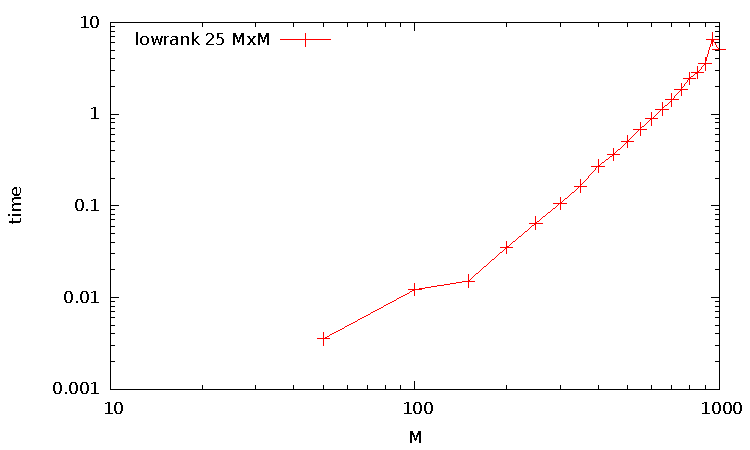
\includegraphics[width=1\textwidth]{lowrankM.pdf}
	\caption{Rekentijd voor matrix product}
	\label{lowrank}
\end{subfigure}
\begin{subfigure}{.48\textwidth}
	\centering
	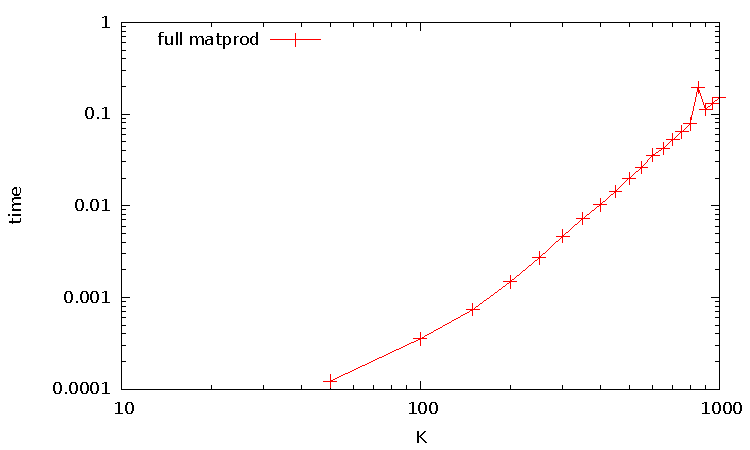
\includegraphics[width=1\textwidth]{fullprod.pdf}
	\caption{Rekentijd voor matrix product}
	\label{fullprod}
\end{subfigure}
\caption{rekencomplexiteit lowrank en matrix product met volledige matrix}
\label{o3complex}
\end{figure}

zoals te zien op Figuur \ref{o3complex} is zowel het product van 2 volledige matrices als het berekenen van een lowrank matrix met een gegeven volledige matrix \(O(n^3)\). Dit is zoals de verwachtingen. Als we beide figuren met elkaar vergelijken kunnen we ook opmerken dat het berekenen van een lagere rang matrix meer tijd vraagt als het product nemen van twee volledige matrices. Dit wil zeggen dat wanneer we 2 matrices willen vermenigvuldigen het weinig zinvol is om eerst een lagere rang matrix te berekenen. Het nut hiervan wordt pas bereikt wanneer we meerdere bewerkingen moeten doen met deze matrix. Daarnaast kunnen we vermelden dat de rekentijd van het berekenen van een lagere rang matrix onafhankelijk is van de rang waarin we ge\"interesseerd zijn. Dit komt omdat we telkens de volledige SVD berekenen met \(O(n^3)\) rekencomplexiteit.

\begin{figure}
\centering
	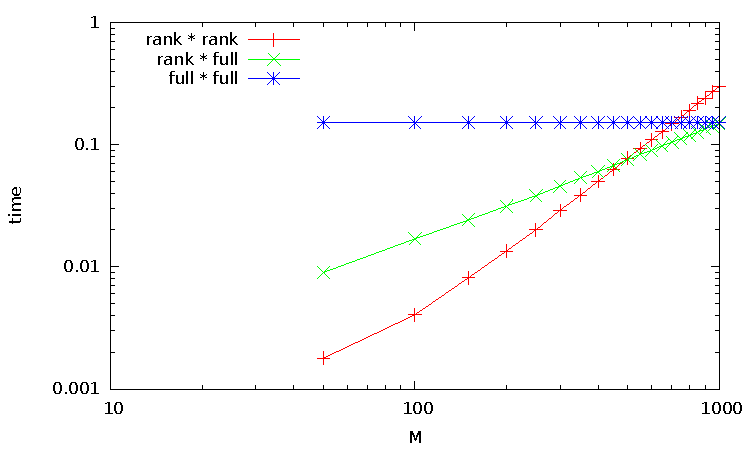
\includegraphics[width=1\textwidth]{rankfull.pdf}
	\caption{Rekentijd voor matrix product van 2 1000x1000 matrices (eventueel van rank-M benadering}
	\label{rankfull}
\end{figure}


\section*{discussie}
\section*{besluit}




\end{document}
